% ==============================================================================
% RESULTADOS
% ==============================================================================
% Instrucciones de la plantilla:
% - Por cada una de las actividades, describir detalladamente los resultados alcanzados, tanto de las solicitadas, como de los experimentos.
% - Incluir capturas de pantalla debidamente tituladas y referenciadas en el texto.
% - REGLA: No se aceptarán solo capturas de pantalla; deben estar explicadas.
% - Analizar ventajas y desventajas de la metodología aplicada.
% ==============================================================================

\section{Resultados}

A continuación se exponen y analizan los resultados obtenidos en cada una de las actividades prácticas y pruebas experimentales.

\subsection{Resultados de la Actividad 1}
En la Actividad 1 se logró la representación gráfica correcta de la escena interactiva. Como se observa en la Figura \ref{fig:resultado_act1}, el cauce de renderizado procesó satisfactoriamente las primitivas geométricas...

% Ejemplo de inserción de figura con título y referencia en el texto:
\begin{figure}[H]
    \centering
    % Coloca tu imagen en la carpeta Imagenes/ y descomenta la siguiente línea:
    % \includegraphics[width=0.75\textwidth]{Imagenes/resultado_actividad1.png}
    % Mientras tanto, un marco de demostración:
    \setlength{\fboxrule}{1pt}
    \framebox[0.75\textwidth]{\rule{0pt}{4cm}\large Captura de pantalla de la Actividad 1}
    \caption{Resultado visual obtenido al ejecutar la escena interactiva de la Actividad 1.}
    \label{fig:resultado_act1}
\end{figure}

\subsubsection{Análisis de ventajas y desventajas}
\begin{itemize}
    \item \textbf{Ventajas:} El enfoque utilizado mediante VAO/VBO optimiza la transferencia de memoria hacia la GPU, reduciendo la sobrecarga de la CPU por llamada de dibujo.
    \item \textbf{Desventajas:} Requiere un manejo explícito del ciclo de vida de los identificadores de recursos en memoria gráfica para prevenir fugas de memoria.
\end{itemize}

\subsection{Resultados de la Actividad 2}
% Describir resultados y capturas para la Actividad 2:
\textit{Describir detalladamente los resultados obtenidos en la segunda actividad y referenciar sus figuras correspondientes...}

\subsection{Resultados de la Actividad 3}
La adaptación en Blender dejó a Exo Gray como un modelo que \texttt{AnimatedModel} puede animar sin modificaciones: una malla, un material y 94 huesos. La Figura \ref{fig:atlas_exogray} muestra el atlas resultante, con el traje en la mitad izquierda y la cara y el cuerpo en la derecha, y la Figura \ref{fig:exogray_blender} muestra el modelo ya unido y animado dentro de Blender antes de exportarlo. Que la cara y el traje se vean en su lugar confirma que el recorrido de las coordenadas UV a cada mitad del atlas fue correcto.

\begin{figure}[H]
    \centering
    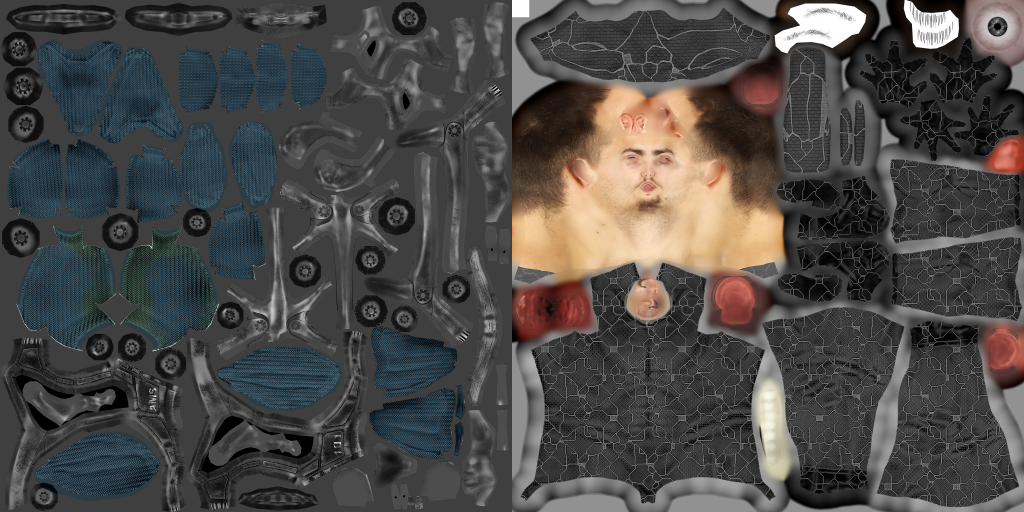
\includegraphics[width=0.75\textwidth]{Imagenes/E3/01_exogray_atlas_texturas.png}
    \caption{Atlas de $4096 \times 2048$ píxeles generado por \texttt{personaje\_act3.py}: a la izquierda la textura del traje y a la derecha la de la cara y el cuerpo.}
    \label{fig:atlas_exogray}
\end{figure}

\begin{figure}[H]
    \centering
    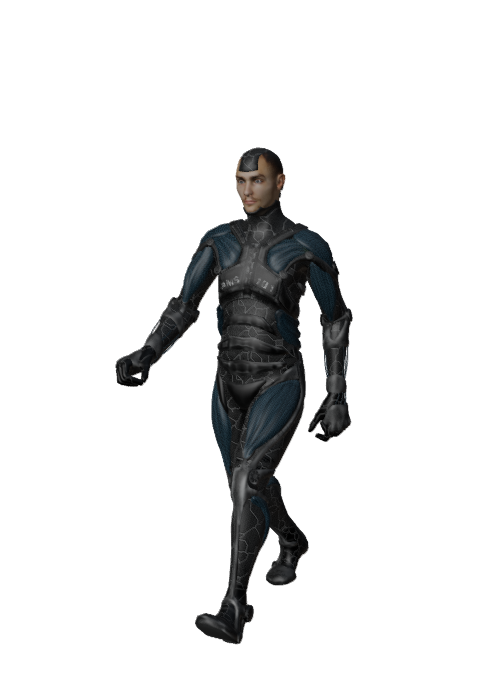
\includegraphics[width=0.32\textwidth]{Imagenes/E3/02_exogray_blender_una_malla.png}
    \caption{Exo Gray en Blender después de la adaptación: una sola malla de 16\,738 vértices con el atlas aplicado, a mitad del ciclo de caminata.}
    \label{fig:exogray_blender}
\end{figure}

En OpenGL el personaje aparece sobre la avenida de enfrente de la ciudad y responde a las cuatro flechas (Figura \ref{fig:exogray_opengl}): las flechas \texttt{Arriba} y \texttt{Abajo} lo desplazan en la dirección hacia la que mira y las laterales lo giran sobre el eje $Y$, mientras la caminata se reproduce en su lugar. Con la tecla \texttt{G} se cambia al personaje de ejemplo del laboratorio (Figura \ref{fig:personaje_clase}), que se mueve con exactamente los mismos controles. Como los dos personajes comparten la posición y la orientación, el cambio ocurre en el mismo punto de la escena.

\begin{figure}[H]
    \centering
    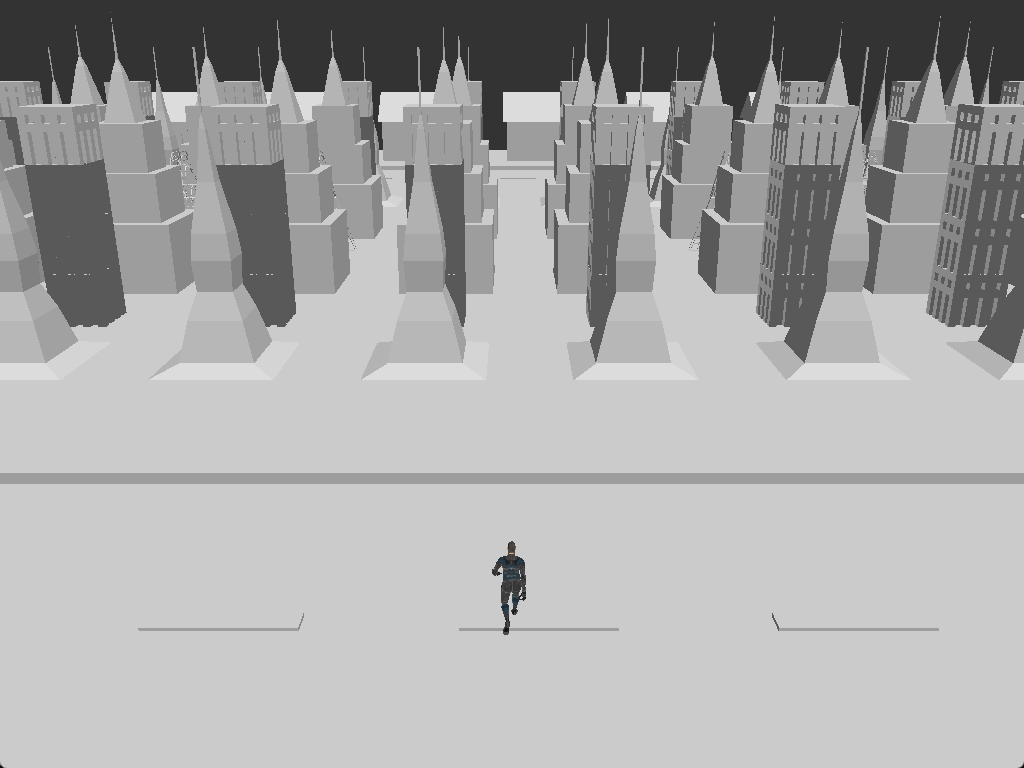
\includegraphics[width=0.75\textwidth]{Imagenes/E3/04_opengl_exogray_ciudad.png}
    \caption{Exo Gray cargado en OpenGL con \texttt{AnimatedModel}, sobre la avenida de enfrente de la ciudad.}
    \label{fig:exogray_opengl}
\end{figure}

\begin{figure}[H]
    \centering
    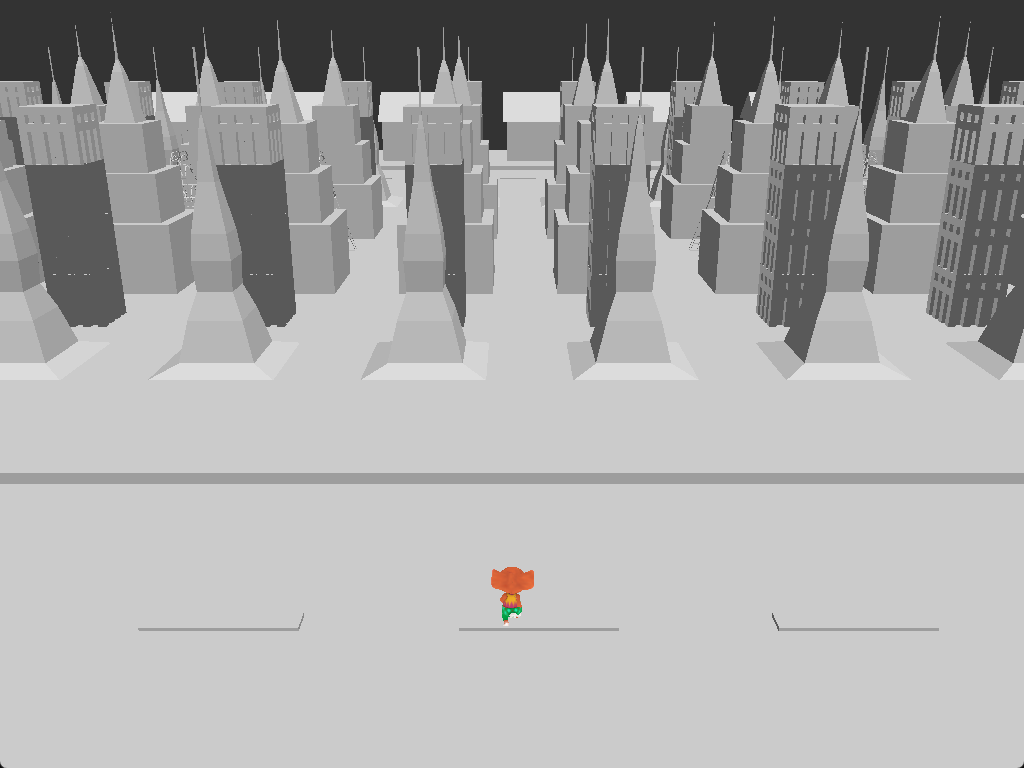
\includegraphics[width=0.75\textwidth]{Imagenes/E3/05_opengl_personaje_clase.png}
    \caption{El personaje de ejemplo del laboratorio (\texttt{character.fbx}) en la misma posición, después de presionar la tecla \texttt{G}.}
    \label{fig:personaje_clase}
\end{figure}

\subsubsection{Análisis de ventajas y desventajas}
\begin{itemize}
    \item \textbf{Ventajas:} Adaptar el modelo en lugar del cargador deja intacta la clase que usan las demás prácticas, y como todo el proceso quedó en un guion, cualquier otro personaje de Mixamo se puede preparar con el mismo procedimiento cambiando solo el archivo de entrada.
    \item \textbf{Desventajas:} El atlas pesa 12 MB y, al juntar las texturas en una sola, cada parte del cuerpo dispone de la mitad de la resolución horizontal que tenía. Además, el tiempo de carga crece mucho con el número de vértices por la forma en que la clase asigna los pesos.
\end{itemize}

\subsection{Resultados de la Actividad 4}
La secuencia del modelado quedó registrada en Blender paso a paso. La Figura \ref{fig:casa_pasos} resume la construcción de la casa: los muros subdivididos en tres columnas, las puertas y ventanas hundidas con \textit{Inset} y \textit{Extrude}, y el techo de dos aguas obtenido al escalar a cero la cara superior de un cubo.

\begin{figure}[H]
    \centering
    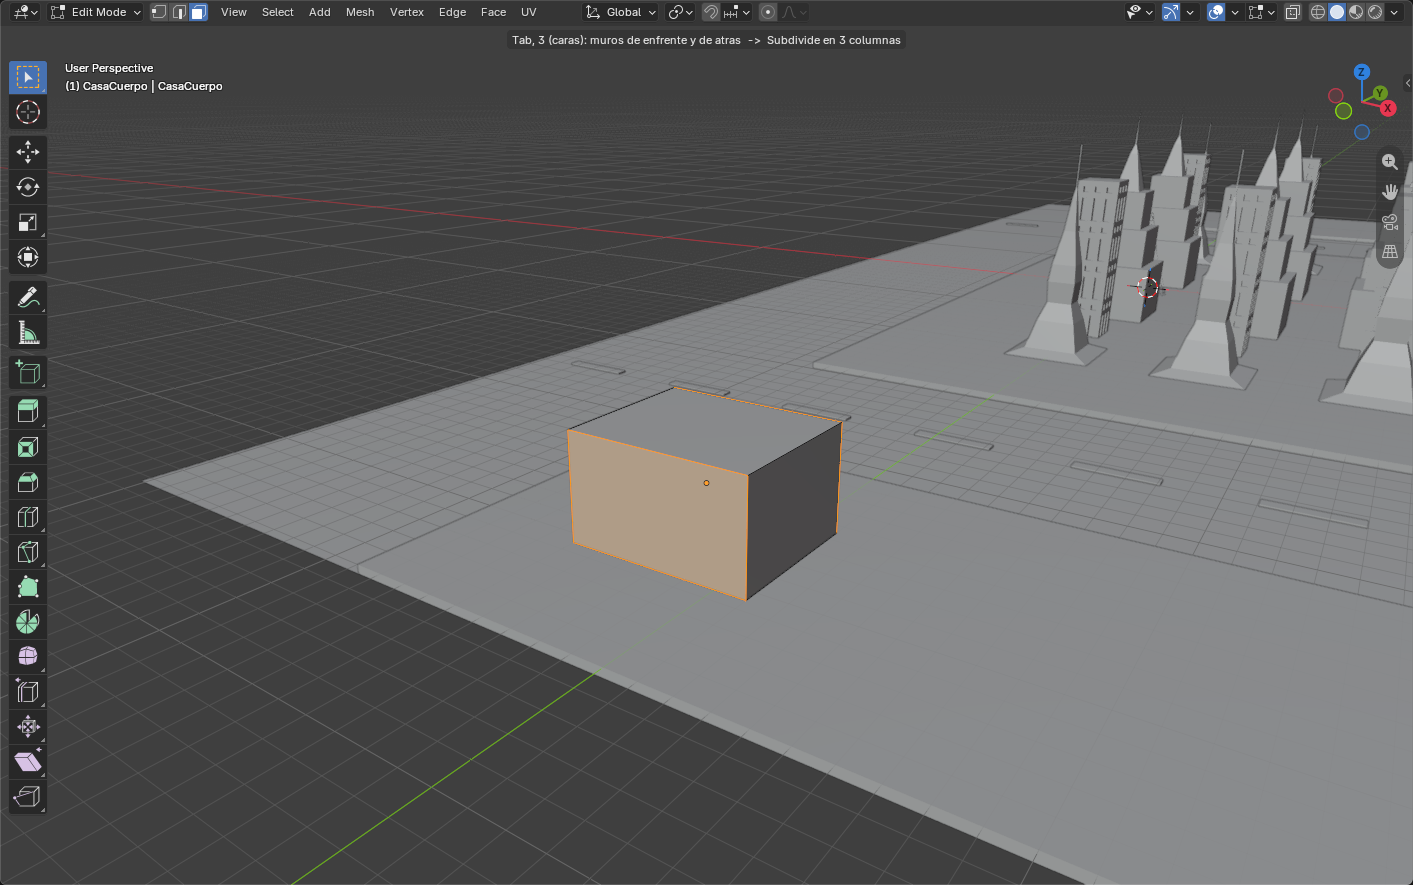
\includegraphics[width=0.32\textwidth]{Imagenes/E4/06_casa_subdivide.png}
    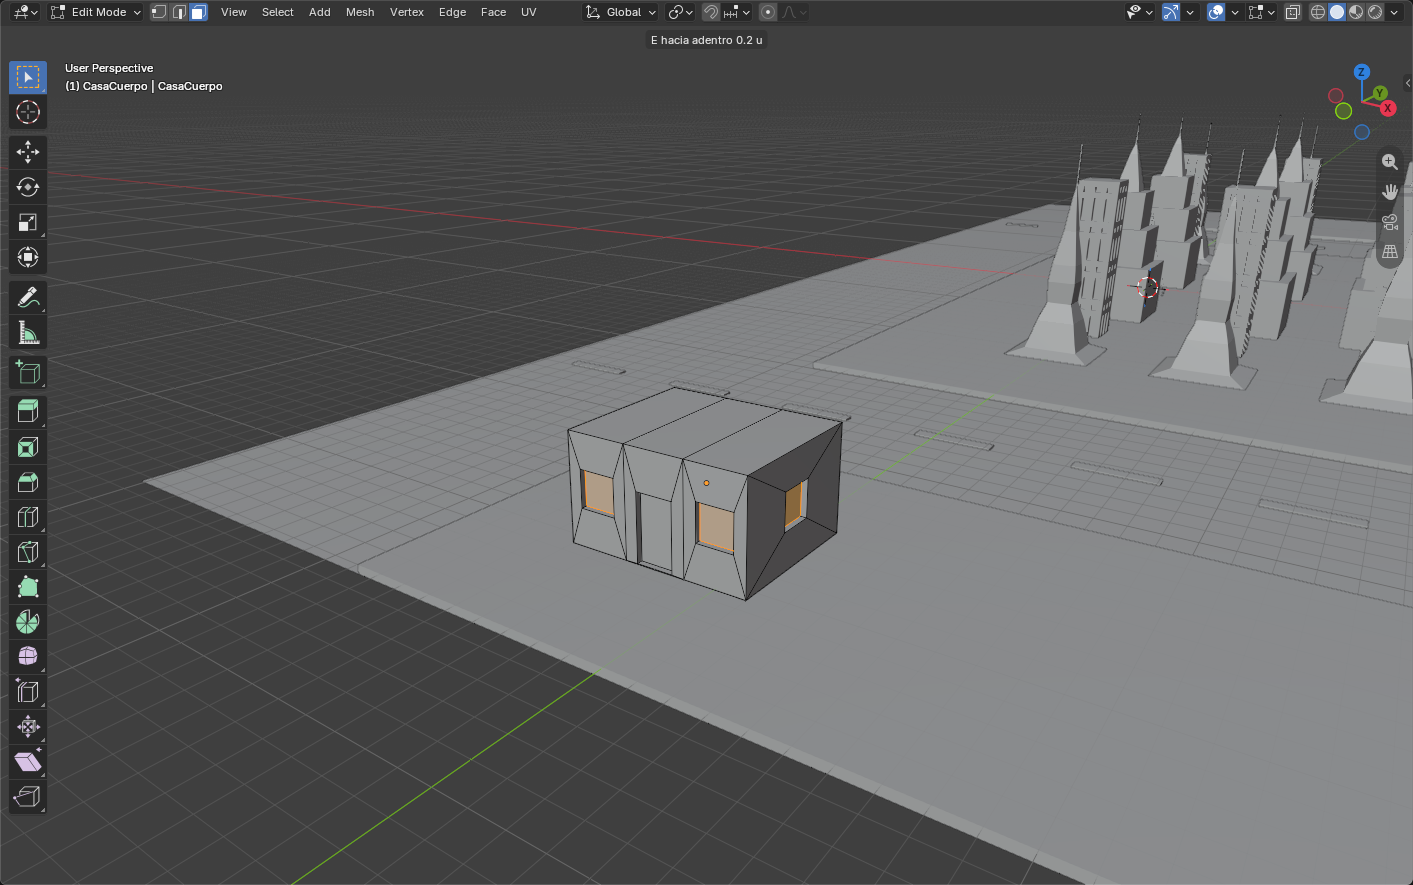
\includegraphics[width=0.32\textwidth]{Imagenes/E4/08_casa_ventanas.png}
    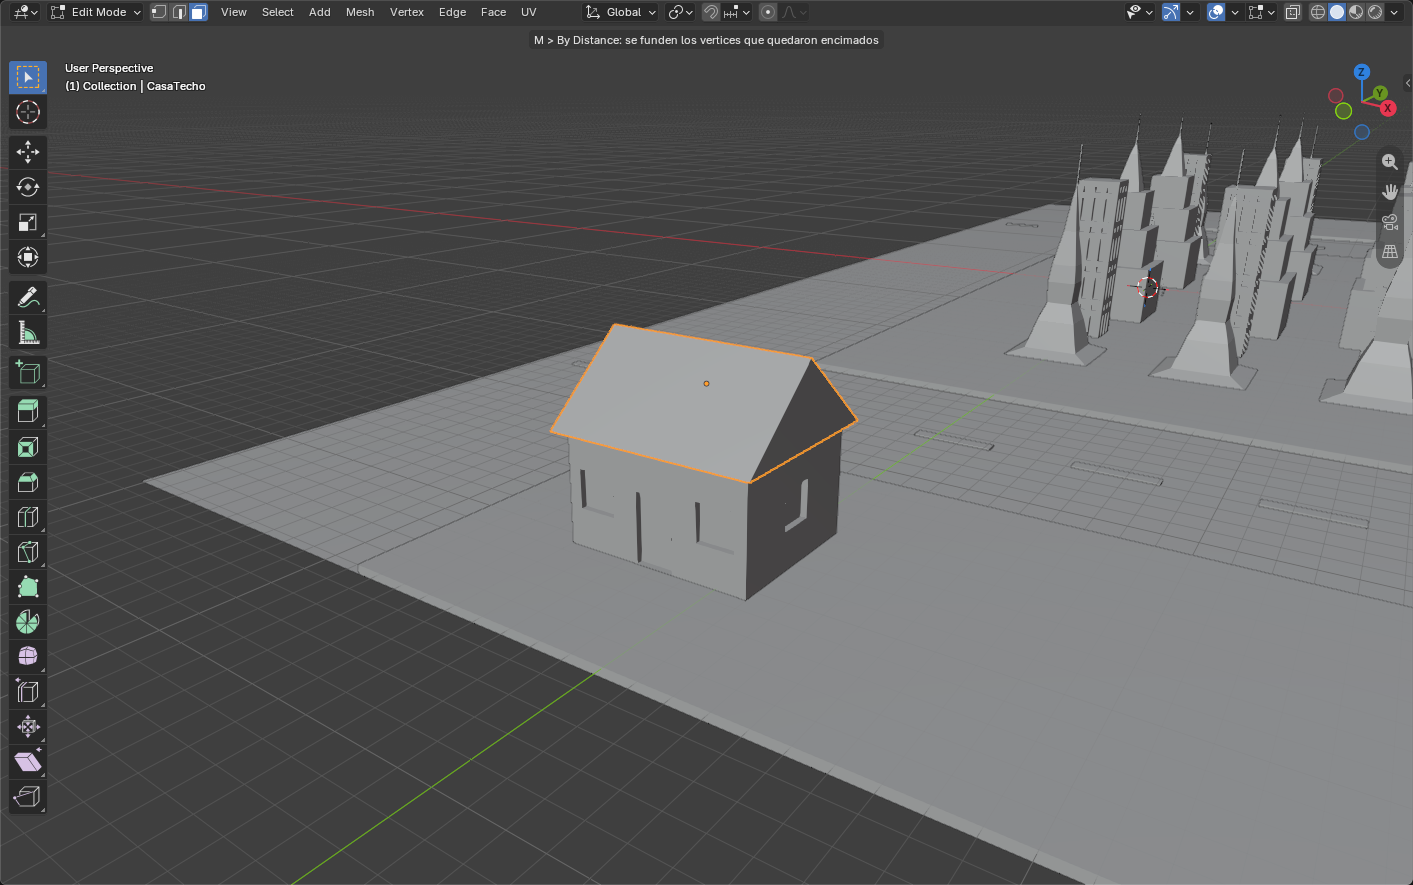
\includegraphics[width=0.32\textwidth]{Imagenes/E4/09_casa_techo_dos_aguas.png}
    \caption{Construcción de la casa: subdivisión de los muros en tres columnas (izquierda), puertas y ventanas hundidas (centro) y techo de dos aguas con \textit{S Y 0} (derecha).}
    \label{fig:casa_pasos}
\end{figure}

La Figura \ref{fig:zona_ampliada} muestra el modelo completo antes de exportarlo: la ciudad de la Actividad 1 sobre su banqueta, las dos avenidas con sus líneas centrales y las dos filas de seis casas, cada una con la puerta hacia su avenida. El archivo exportado, \texttt{Ciudad.fbx}, pesa 6.3 MB.

\begin{figure}[H]
    \centering
    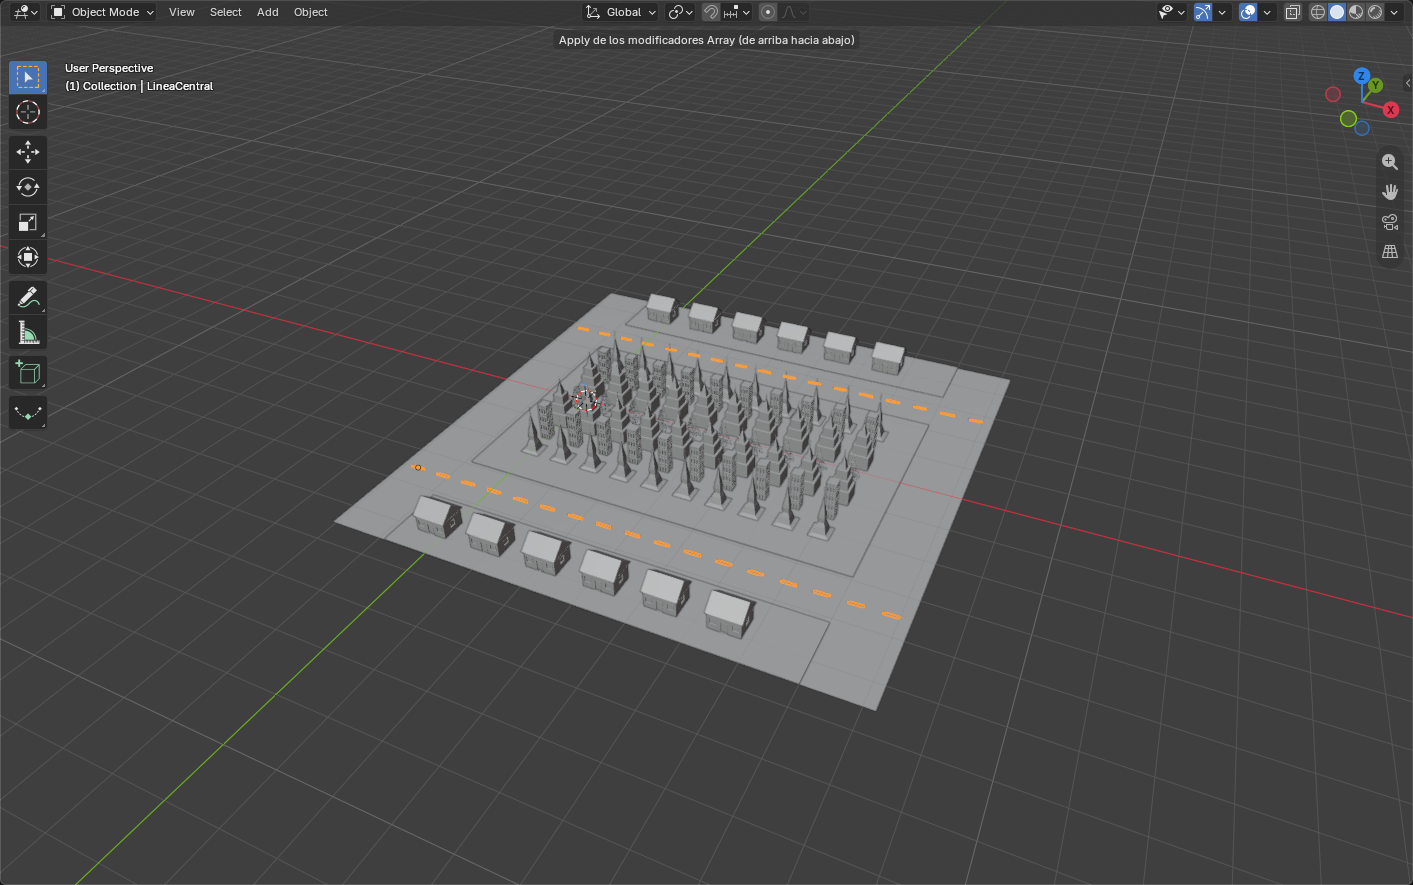
\includegraphics[width=0.8\textwidth]{Imagenes/E4/11_zona_ampliada.png}
    \caption{Zona ampliada en Blender: manzana central con los edificios, avenidas de enfrente y de atrás con sus líneas centrales y dos filas de casas.}
    \label{fig:zona_ampliada}
\end{figure}

Cargado en OpenGL, el modelo se ve completo desde la avenida (Figura \ref{fig:ciudad_opengl}). Sin usar colores, la diferencia de altura entre banqueta y asfalto y la luz direccional del \textit{shader} gris bastan para distinguir la calle, el borde de la banqueta y las caras de cada edificio. Al recorrer la escena con el personaje, la avenida y las calles laterales permiten rodear toda la manzana de los edificios.

\begin{figure}[H]
    \centering
    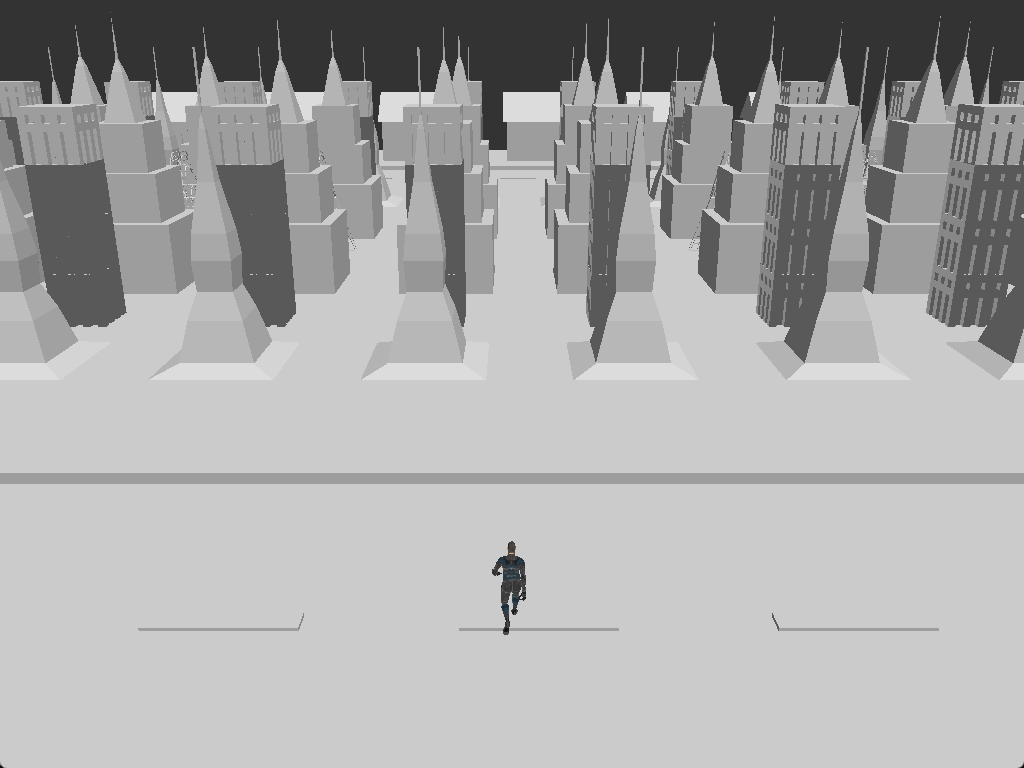
\includegraphics[width=0.75\textwidth]{Imagenes/E4/13_opengl_ciudad_ampliada.png}
    \caption{Ciudad.fbx en OpenGL con el \textit{shader} gris, vista desde la avenida de enfrente.}
    \label{fig:ciudad_opengl}
\end{figure}

\subsubsection{Análisis de ventajas y desventajas}
\begin{itemize}
    \item \textbf{Ventajas:} Al calcular el trazo desde la caja de la ciudad, el procedimiento se adaptó sin cambios a un modelo de otro tamaño, y el uso de \textit{Array} hace que agregar o quitar casas sea cuestión de cambiar un solo número.
    \item \textbf{Desventajas:} Como todo se exporta en un solo FBX con un solo material, en OpenGL la ciudad, las casas y las calles comparten el mismo \textit{shader} y no pueden tratarse por separado; además, las casas son copias idénticas, así que la zona se ve repetitiva.
\end{itemize}